\section{Estimating associations between DNA methylation and gene expression} \label{sec:mt}

\ifpdf
    \graphicspath{{Chapter3/mt/Figs/Raster/}{Chapter3/mt/Figs/PDF/}{Chapter3/mt/Figs/}}
\else
    \graphicspath{{Chapter3/mt/Figs/Vector/}{Chapter3/mt/Figs/}}
\fi

We have shown that scBS-seq enables the exploration of intercellular heterogeneity in DNA methylation genome-wide. To further study the relationship between heterogeneity in DNA methylation and gene expression, we developed scM\&T-seq, a protocol for parallel profiling of DNA methylation and gene expression in single cells. In combination with scM\&T-seq, we developed methods for estimating associations between DNA methylation and gene expression in single cells, which will be described in the following.

\subsection{Parallel single-cell DNA methylation and gene expression profiling}

\citet{macaulay_g&t-seq:_2015} have recently developed G\&T-seq, a method for parallel genome and transcriptome sequencing within single cells. Importantly, G\&T-seq utilizes physical separation of RNA and DNA allowing bisulfite conversion of DNA without affecting the transcriptome. We now apply scBS-seq to genomic DNA purified according to the G\&T-seq protocol. Our scM\&T-seq protocol consists of isolating single cells, followed by physical separating DNA and RNA using the G\&T protocol (\Cref{fig:mt_proto}). DNA is bisfulfite treated and sequenced using scBS-seq to quantify DNA methylation of individual cells, and RNA is sequenced using scRNA-seq~\citep{jaitin_massively_2014} to quantify gene expression.

\begin{figure}[htbp!]
  \begin{minipage}[c]{0.65\textwidth}
    \centering
    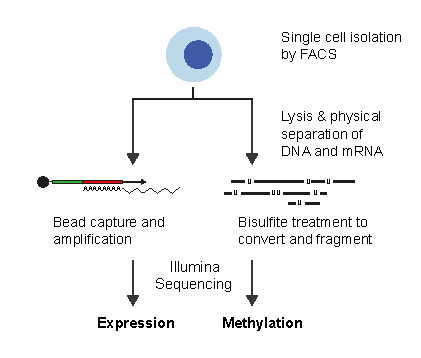
\includegraphics[width=1.0\textwidth]{proto}
  \end{minipage}
  \begin{minipage}[c]{0.32\textwidth}
    \caption[Schematic overview of the scM\&T-seq protocol.]{Schematic overview of the scM\&T-seq protocol. Single-cells are isolated by FACS sorting and extracted DNA separated from RNA using G\&T-seq. DNA is treated with bisulfite and sequenced using scBS-seq to quantify DNA methylation; RNA is amplified and sequences to quantify gene expression.}
    \label{fig:mt_proto}
  \end{minipage}
\end{figure}

We evaluated scM\&T-seq on mouse ESCs. In the presence of serum, these cells are characterized by high transcriptional and epigenetic heterogeneity. To investigate the link between epigenetic and transcriptional heterogeneity in ESCs, we performed scM\&T-seq on 76 individual serum ESCs and 16 ESCs grown in `2i' media, which induces genome-wide DNA hypomethylation.

To assess the quality of the scBS-seq data, we compared the resulting single-cell methylomes with the 20 serum and 12 2i ESCs that we profiled with stand-alone scBS-seq (\Cref{sec:bs_proto}). The genome-wide CpG coverage at matched sequencing depth was consistent across scM\&T-seq and scBS-seq (\Cref{fig:mt_qc}~(a)) and we found that scM\&T-seq covered a large proportion of sites in different genomic contexts with sufficient frequency to enable the analysis of epigenome heterogeneity across cells. As additional validation, we assessed the discrimination of serum and 2i ESCs by both stand-alone scBS-seq and scM\&T-seq, finding a similar degree of separation that was consistent with bulk datasets published previously~\citep{ficz_fgf_2013} (\Cref{fig:mt_qc}~(b)), with similar conclusions when using a joint hierarchical clustering across all cells (\Cref{fig:mt_clust}). Notably, the difference between protocols and biological batches had a substantially smaller effect (PC2, 3\% variance) than cell type differences (PC1, 48\% variance), and by combining data across cells, we found that both protocols yield genome-wide methylation profiles that accurately recapitulate bulk methylation profiles in the same cell type (\Cref{fig:mt_bulk}). Finally, we compared estimates of methylation heterogeneity in different genomic contexts, again finding good agreement between protocols (\Cref{fig:mt_var}). Taken together, these analyses provide confidence that the parallel scM\&T-seq method yields results that are in agreement with data from stand-alone scBS-seq.

\citet{macaulay_g&t-seq:_2015} has previously shown that the scRNA-seq data generated by the G\&T-seq method is of similar quality to that generated using the scRNA-seq protocol. We obtained an average of 2.7 million scRNA-seq reads per cell, and we excluded cells with fewer than 2 million mapped reads. In ESCs that met scRNA-seq quality-control criteria, we detected transcripts from between 4000 and 8000 genes exceeding one transcript per million, consistent with previous measurements made using the method (\Cref{fig:mt_qc_rna}).

\begin{figure}[htbp!]
\centering
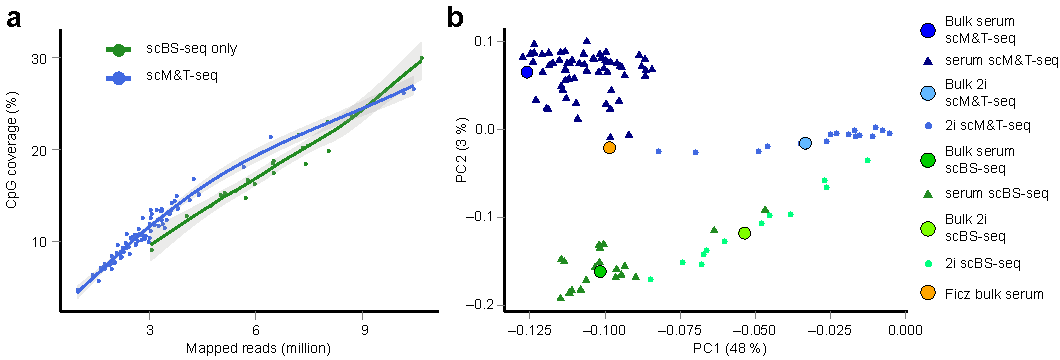
\includegraphics[width=1.0\textwidth]{qc}
\caption[Quality controls of scM\&T-seq protocol.]{Schematic overview of the scM\&T-seq protocol. (a) CpG coverage of single cells as a function of the number of mapped sequencing reads. Green: stand-alone scBS-seq, Blue: scM\&T-seq. (b) Joint principal component analysis of the methylomes (gene body methylation) of 61 serum ESCs (dark blue) and 16 2i ESCs (light blue) obtained using scM\&T-seq, as well as 20 serum ESCs (green) and 12 2i ESCs (yellow) sequenced using stand-alone scBS-seq. The solid circles correspond to synthetic bulk datasets form the same cells. For comparison, we also included a bulk serum ESC DNA methylation dataset~\citep{ficz_fgf_2013} (orange). Cell type explained a substantially larger proportion of variance (PC1, 48\%) than protocol (PC2, 3\%).}
\label{fig:mt_qc}
\end{figure}

For subsequent analyses, we focused on serum ESCs only since transcription and DNA methylation are uncoupled in 2i ESCs~\citep{ficz_fgf_2013,habibi_whole-genome_2013}. A comparison of the principal components derived from gene body methylation and gene expression revealed associations between some factors of variations of both data modalities (\Cref{fig:mt_cca}; \Cref{fig:mt_cca_cor}). However, a hierarchical clustering analysis of gene body methylation and gene expression for the 300 most variable genes revealed distinct clustering of cells when using either source of information (\Cref{fig:mt_heat}). This suggests that global methylome and transcriptome profiles yield complementary but distinct aspects of cell state. This is also consistent with previous observations that the transcriptome and methylome are partially uncoupled in serum ESCs~\citep{ficz_fgf_2013}.

\begin{figure}[htbp!]
\centering
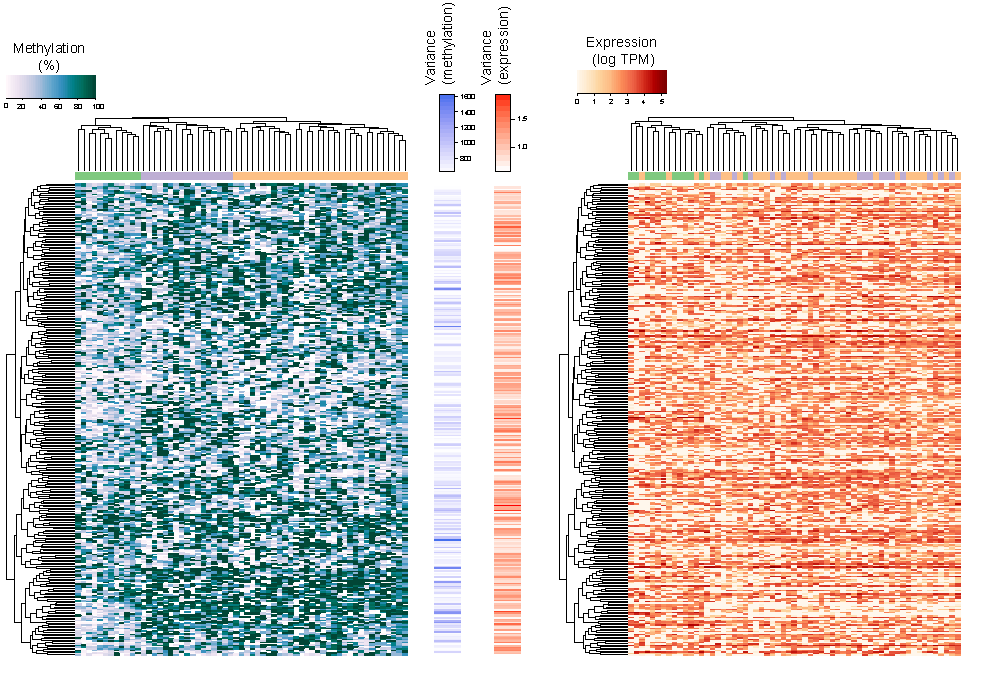
\includegraphics[width=1.0\textwidth]{heat}
\caption[Clustering analysis of transcriptome and methylome data.]{Clustering analysis of transcriptome and methylome data from 61 serum ESCs, considering gene body methylation (left) and gene expression (right) for the 300 most heterogeneous genes (based on gene body methylation). The order of genes was taken from an individual clustering analysis based on gene body methylation whereas cells were clustered separately either using DNA methylation or expression data, and coloured by methylation cluster. The bar plots in the center show the heterogeneity in DNA methylation (left) and gene expression (right).}
\label{fig:mt_heat}
\end{figure}


\subsection{Methods for estimating associations between DNA methylation and gene expression} \label{sec:mt_method}

\newcommand{\Xcov}{\operatorname{cov}}
\newcommand{\Xcor}{\operatorname{cor}}

\begin{figure}[htbp!]
\centering
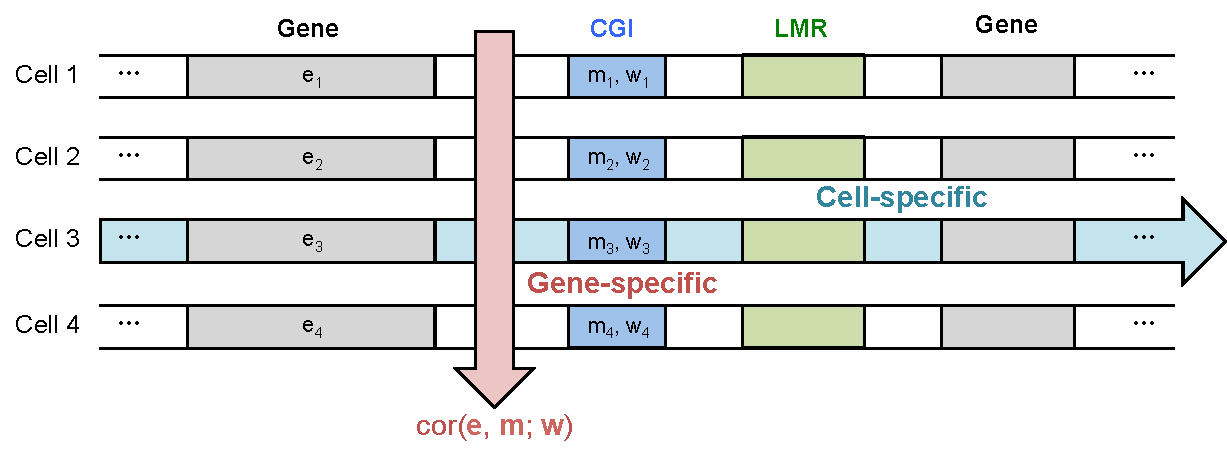
\includegraphics[width=1.0\textwidth]{method}
\caption[Schematic representation cell-specific and gene-specific correlation analysis between methylome and transcriptome.]{Schematic representation cell-specific and gene-specific correlation analysis between methylome and transcriptome. Cell-specific analysis is performed for a single cell or a bulk population of cells across multiple genes. Gene-specific analysis is performed for a single gene across multiple cells. The vector $e$ represents the expression rates of the considered gene for all cells, $m$ the mean methylation rates in the corresponding genomic context, and $w$ the number of covered CpG sites within that context. Associations were estimated by the weighted Pearson correlation $\Xcor(e, m; w)$ to account for differences in CpG coverage between cells.}
\label{fig:mt_method}
\end{figure}

Previous studies on data from bulk sequencing protocols estimated correlations between methylome and transcriptome in a bulk population of cells across multiple genes (\Cref{fig:mt_method}). In contrast, scM\&T-seq separates individual cells and hence enables estimating associations for a particular gene across multiple cells. Let $e$ be a vector with expression rates of cells for a particular gene, $m$ be methylation rates of the associated region, and $w$ be weights corresponding to the number of covered CpGs sites within the region. Then we estimated associations using weighted Pearson correlation $\operatorname{cor}(e,m;w)$ between gene-expression $e$ and methylation $m$:
\begin{align} \label{eq:mt_wcor}
  \Xcor(e,m;w)=\frac{\Xcov(e,m;w)}{\sqrt{\Xcov(e,e;w)\Xcov(m,m;w)}}
\end{align}
Here, $\Xcov(x,y;w)$ is the weighted covariance
\begin{align}
  \Xcov(x,y;w)=\sum_i \frac{w_i (x_i-m(x;w))(y_i-m(y;w))}{\sum_i w_i },
\end{align}
and $m(x;w)$ the weighted arithmetic mean:
\begin{align}
  m(x;w)=\frac{\sum_i x_i w_i}{\sum_i w_i}
\end{align}
By computing weighted correlations, we accounted for differences in CpG coverage between cells. We considered all possible relationships between genes and methylated regions within 10~kbp of the gene (upstream and downstream of gene start or stop). We performed two-sided Student's t-tests to test for non-zero correlations, and adjusted p-values for multiple testing for each context using the Benjamini-Hochberg procedure.

We considered gene expression levels on a logarithmic scale using log10 normalized TPM counts. We estimated binary single-base pair CpG methylation states by the ratio of methylated read counts to total read counts. We further estimated the methylation rate in different genomic contexts, such as gene body, promoter, or enhancer annotations, as the mean CpG methylation rate within the region defined by the context.

We discarded genes with low expression levels or low expression and methylation variability between cells, following the rational of independent filtering~\citep{bourgon_independent_2010}. First, a minimum expression level (at least 10 TPM counts) in at least 10\% of all cells was required. From these, the 7500 most variable genes were considered for analysis. Second, methylated regions were required to be covered by at least one read in at least 50\% of all cells.


\subsection{Associations between DNA methylation and gene expression in different genomic contexts} \label{sec:mt_results}

Using weighted Pearson correlation (\Cref{eq:mt_wcor}), we tested for associations between expression of individual genes and DNA methylation variation at several genomic contexts. We identified a total of 1493 associations ($\FDR<0.1$; \Cref{fig:mt_gene_volcano}), which were robust when using a bootstrapping approach to subsample the set of cells. We found both positive and negative associations, highlighting the complexity of interactions between the methylome and transcriptome~\citep{dey_integrated_2015}. While methylation of non-CGI promoters is known to be associated with transcriptional repression, the role of enhancer methylation is less clear. Accordingly, negative correlations between DNA methylation and gene expression were predominant for non-CGI promoters, whereas positive and negative associations were more balanced in distal regulatory elements including LMRs (\Cref{fig:mt_gene_volcano}; \Cref{fig:mt_gene_r}; \Cref{fig:mt_gene_volcano_all}). Interestingly, associated genes were enriched for known pluripotency and differentiation genes~\citep{kolodziejczyk_single_2015} ($\FDR<0.01$, Fisher's exact test). Our results provide the first evidence that heterogeneous methylation of distal regulatory elements, e.g. LMRs, accompanies heterogeneous expression of key pluripotency factors in stem cell populations~\citep{lee_reprogramming_2014}.

\begin{figure}[htbp!]
\centering
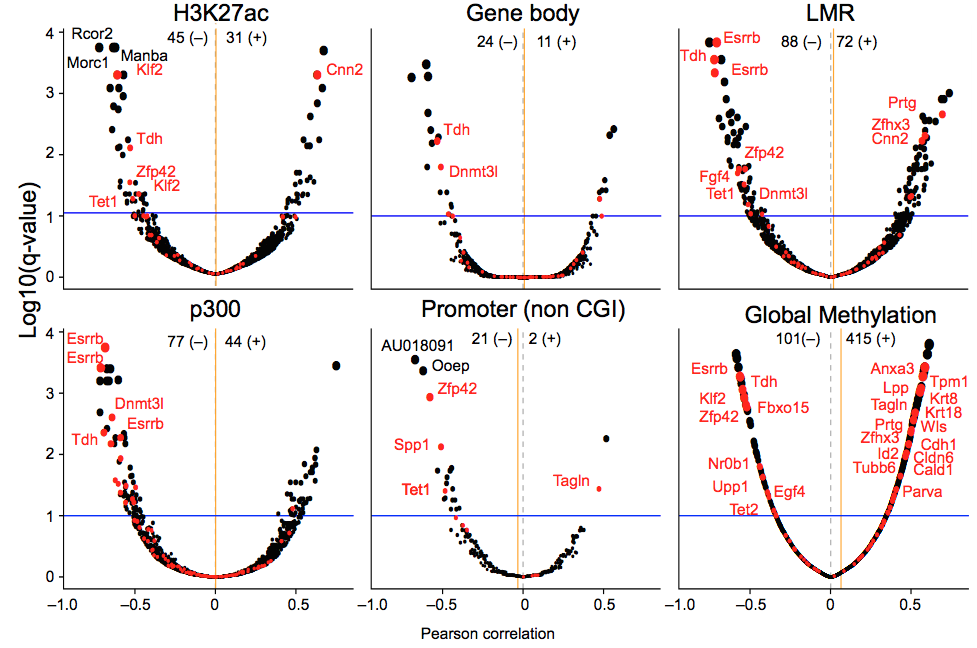
\includegraphics[width=0.8\textwidth]{gene_volcano}
\caption[Volcano plots of correlation coefficients.]{Volcano plots of correlation coefficients (Pearson's $r^2$) from association tests between gene expression heterogeneity of individual genes and DNA methylation heterogeneity in alternative genomic contexts. Shown is the correlation coefficient for every gene (x-axis) versus the adjusted p-value (using Benjamini-Hochberg correction; y-axis). The size of dots corresponds to the adjusted p-value. A set of 86 known pluripotency and differentiation genes are highlighted in red. The blue horizontal line corresponds to the $\FDR=0.1$ significance threshold. The total number of significant positive (+) and negative (–) correlations ($\FDR<0.1$) for each annotation is shown in the header of each panel. The orange vertical bar corresponds to the average correlation coefficient across all genes for a given context.}
\label{fig:mt_gene_volcano}
\end{figure}

As an example, \cref{fig:mt_zoom} shows the association map of Esrrb--a known key regulator gene in pluripotency networks~\citep{papp_pluripotency_2012}. Expression of Esrrb negatively correlated with the methylation of several LMR and p300 sites overlapping `super enhancers' in the genomic neighbourhood~\citep{whyte_master_2013}, providing evidence for the regulatory importance of Esrrb. We also found 516 genes whose expression correlated with the overall methylation level ($\FDR<0.1$), indicating substantial links between transcriptional heterogeneity and global methylation levels (\Cref{fig:mt_gene_volcano}).

\begin{figure}[htbp!]
\centering
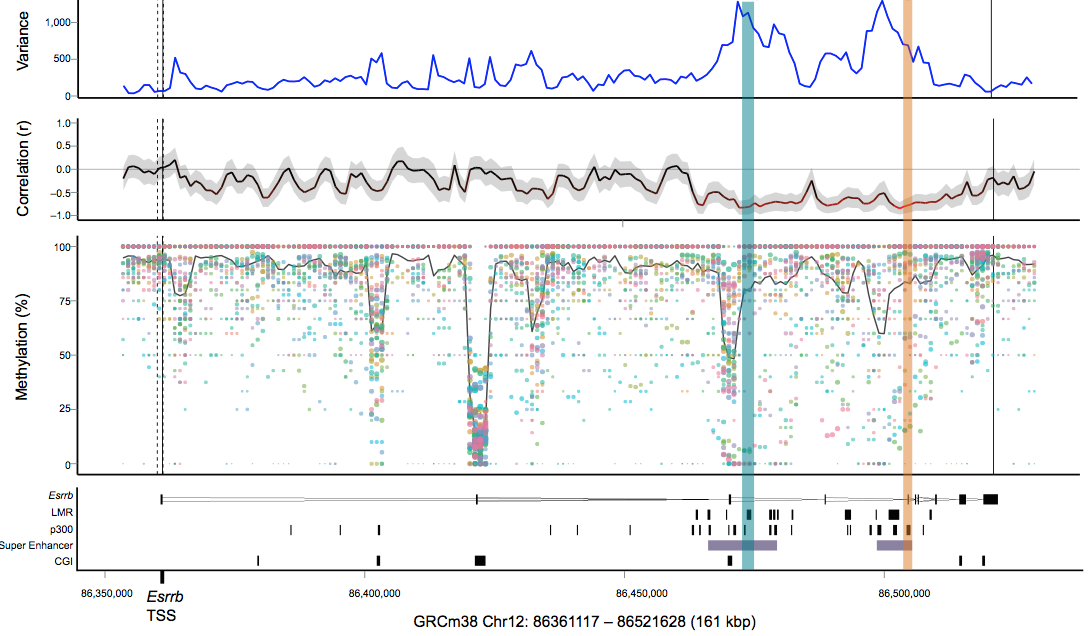
\includegraphics[width=1.0\textwidth]{zoom}
\caption[Representative zoom-in view for the gene Esrrb.]{Representative zoom-in view for the gene Esrrb. From bottom to top, shown is: the annotation of the Esrrb locus with LMR, p300, super enhancer and CGI sites indicated; the estimated methylation rate of $3~kbp$ windows for each cell with the size of dots representing the CpG coverage and the solid line indicating the weighted mean methylation rate across all cells; the correlation between the methylation rate and Esrrb expression for each region coloured by the strength of the correlation and with the shaded area corresponding to the 95\% confidence interval of the correlation coefficient; and the estimated weighted DNA methylation variance between cells. The vertical bars denote the location of a p300 (yellow) and LMR (blue) region, in which DNA methylation is significantly associated with gene expression.}
\label{fig:mt_zoom}
\end{figure}

In addition to between-cell analyses, scM\&T-seq can be used to correlate the methylome and transcriptome between genes in individual cells (\Cref{fig:mt_method}; \Cref{fig:mt_cell}), analogously to studies in cell populations. We found that correlation between methylation and gene expression varied substantially between cells but was consistent in direction with matched RNA-seq and BS-seq data from a population of cells~\citep{ficz_fgf_2013}. Again, this attests to scM\&T-seq being sufficiently accurate to reliably study epigenome-transcriptome linkages. Our results also point to the possibility of heterogeneity between cells in the degree of coupling between the methylome and the transcriptome. Although we have ruled out obvious confounding factors, such as average methylation rate and sequence coverage (\Cref{fig:mt_cell_r_mean}; \Cref{fig:mt_cell_r_cov}), more data will be required to understand possible technical components in these linkages.

\begin{figure}[htbp!]
\centering
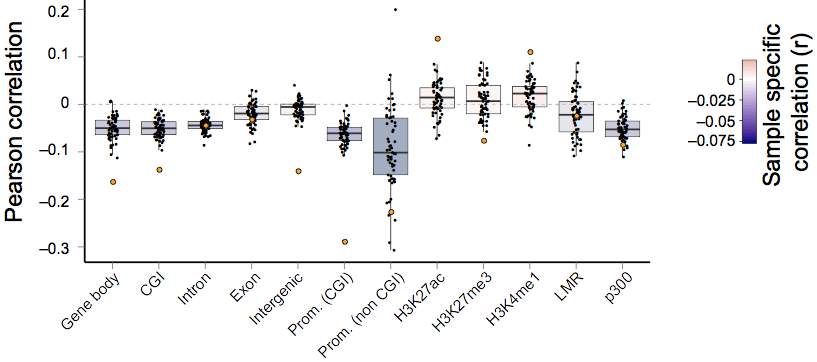
\includegraphics[width=1.0\textwidth]{cell}
\caption[Cell-specific correlation analysis]{Cell-specific association analysis, estimating correlations between DNA methylation in different genomic contexts and gene expression in individual cells. For each annotation, shown are box plots of methylation-expression correlations for all variable genes in single cells, with the correlation obtained from matched RNA-seq and BS-seq of a bulk cell population superimposed (orange circles).}
\label{fig:mt_cell}
\end{figure}
